\documentclass[conf]{new-aiaa}
%\documentclass[journal]{new-aiaa} %for journal papers
%\documentclass[a4paper]{article}
%\documentclass{homework}

%% Sets page size and margins
%\usepackage[a4paper,top=3cm,bottom=2cm,left=3cm,right=3cm,marginparwidth=0.8.75cm]{geometry}

%\usepackage[utf8]{inputenc}
\usepackage{graphicx}
\usepackage{amsmath}
\usepackage[version=4]{mhchem}
\usepackage{siunitx}
\usepackage{longtable,tabularx}
\setlength\LTleft{0pt} 
%======================================

% additions
\graphicspath{ {figures/} }
\usepackage{floatrow}
\usepackage{ar}
\usepackage{amstext} % for \text macro
\usepackage{array}   % for \newcolumntype macro
\usepackage{gensymb} % for degree symbol
\newcolumntype{L}{>{$}l<{$}} % math-mode version of "l" column type
\usepackage[numbered,framed]{matlab-prettifier}

\pagestyle{empty}

\definecolor{listinggray}{gray}{0.9}
\definecolor{lbcolor}{rgb}{0.9,0.9,0.9}
\lstset{
backgroundcolor=\color{lbcolor},
    tabsize=4,    
%   rulecolor=,
    language=fortran,
        basicstyle=\mlttfamily,
        upquote=true,
        aboveskip={1.5\baselineskip},
        columns=fixed,
        showstringspaces=false,
        extendedchars=false,
        breaklines=true,
        prebreak = \raisebox{0ex}[0ex][0ex]{\ensuremath{\hookleftarrow}},
        frame=single,
        numbers=left,
        showtabs=false,
        showspaces=false,
        showstringspaces=false,
        identifierstyle=\mlttfamily,
				keywordstyle=\color{blue}\mlttfamily,
				stringstyle=\color{red}\mlttfamily,
				commentstyle=\color[RGB]{34,139,34}\mlttfamily,
				morecomment=[l][\color{magenta}]{\#}
        %keywordstyle=\color[rgb]{0,0,1},
        %commentstyle=\color[rgb]{0.026,0.112,0.095},
        %stringstyle=\color[rgb]{0.627,0.126,0.941},
        %numberstyle=\color[rgb]{0.205, 0.142, 0.73},
%        \lstdefinestyle{C++}{language=C++,style=numbers}’.
}
%\usepackage{titlesec}
%\titleformat*{\paragraph}{\large\bfseries}
%======================================
\title{CE 791 HPC - Assignment 6\\Matrix Vector Product and Monte-Carlo Integration}

\author{Andrew Navratil}

\begin{document}

\maketitle

\section*{Part 1: Matrix vector product}

Parallel MPI code is written in Fortran to perform a basic matrix vector product using the master-slave paradigm and algorithm from lecture.  Sample code in lecture was utilized as a basis.  Mflops calculation was added, where 2 operations per matrix entry (rows*cols) were estimated (one for the += nd one for the *) in the dot product calculation.  A condition was also put in to handle the receive of MPI\_BOTTOM and break from the slave execution, as the sample code was hanging after calling another receive (could not figure out how it was working, so just put in a conditional to exit when row received from master was 0).  MPI timing was also put in.

Plots for Mflops versus number of processors is shown below.  The number of processors used starts at 2, as the code was not currently setup to only execute on one node, which would be both master and slave.   We can see how this algorithm, that is known to be poor, does not improve with the number of processors, in addition to it's other downfalls.  We also note how improvement does increase with the larger matrix size of 1000x1000 on both clusters.  The actual Mflops value could vary quite a bit on subsequent runs, and the most common / average value was used here.

Three ideas are given for improvement.  One is to decompose the matrix so the entire matrix does not need to be stored on the master node, and use an algorithm for whichever decomposition is chosen.  Second is to send chunks of rows at a time so the communication penalty is not incurred too often.  With a basic calculation as we have here, the MPI communication could easily become the bottleneck if only a single row is sent at a time.  This would result in less load balancing, but likely better overall performance.  Third suggestion is to utilize the MPI topology functions to spread the load better, such as MPI\_DIMS and MPI\_CART related functions.

\begin{figure}[H]
	\centering
	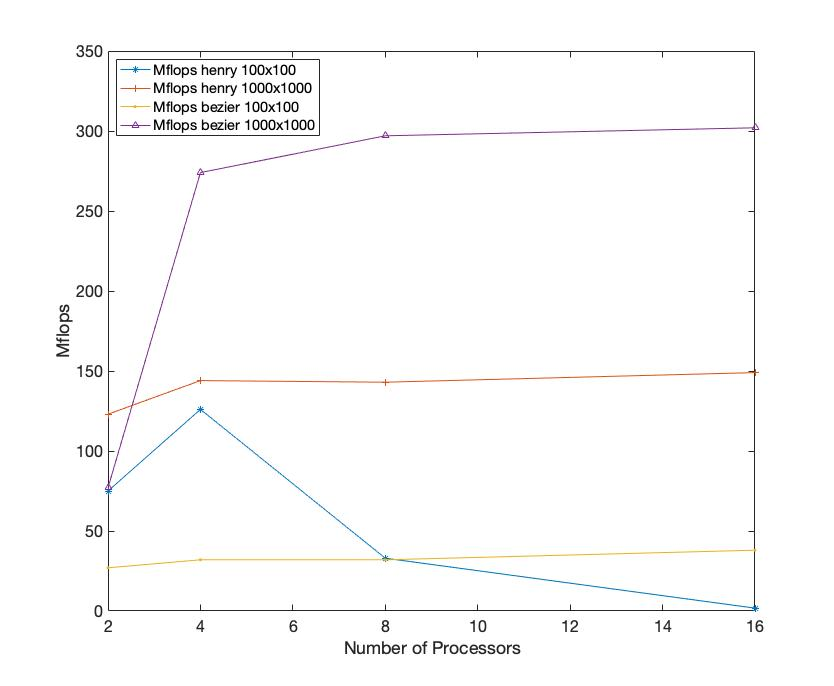
\includegraphics[width=.75\columnwidth]{../hw6data/matvet.jpg}
	\caption{Mflops vs Num Procs for Matrix Vector Product}
\end{figure}

\section*{Part 2: Monte-Carlo integration for calculating PI}

Parallel MPI code is written in Fortran to perform a Monte-Carlo integration to calculate the alue of PI using the master-slave paradigm and algorithm from lecture.  Sample code in lecture was utilized as a basis, converting the C code into Fortran.  Mflops calculation was added with MPI timing calls, where 12 operations per point was estimated.  A different random number generation technique was utilized due to problems with the method from water\_supply\_vector, using random\_seed() and random\_number() functions instead of seed() and rand().  The data type for passing the rands() array from master to workers was changed from MPI\_INT to MPI\_DOUBLE\_PRECISION.  The epsilon value utilized is 0.001 with a CHUNKSIZE of 1000.

Plots for Mflops versus number of processors is shown below, again starting at 2 procs.  We again don't see much improvement in the Mflops when number of processors is increased, as expected, where the primary goal was practice with the MPI groups and the manager-worker paradigm.  

\begin{figure}[H]
	\centering
	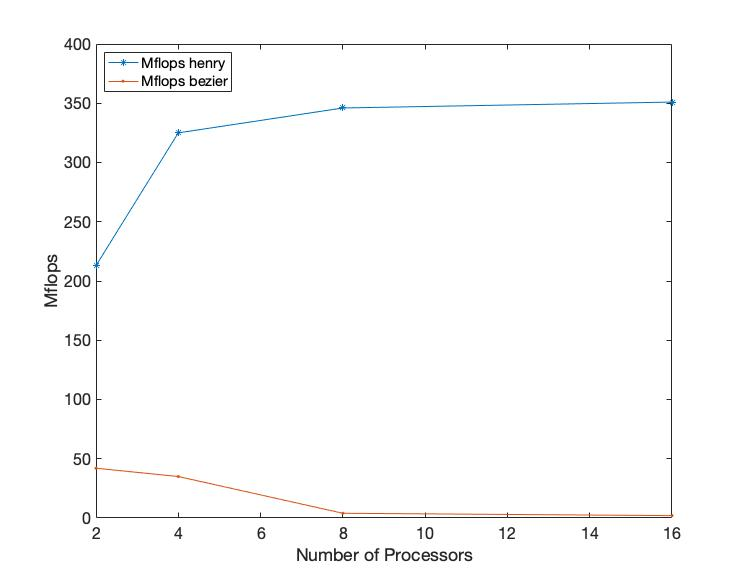
\includegraphics[width=.75\columnwidth]{../hw6data/mc.jpg}
	\caption{Mflops vs Num Procs for Monte-Carlo Pi}
\end{figure}

%======================================
\newpage

\section*{Fortran Code: Matrix Vector Product}
\lstinputlisting[language=fortran]{../a6/matvet.f90}

\newpage

\section*{Fortran Code: Monte-Carlo Pi}
\lstinputlisting[language=fortran]{../a6/mc.f90}

\newpage

\section*{Matlab Code}

\lstset{
  style      = Matlab-editor,
  basicstyle = \mlttfamily,
}
\lstinputlisting{../hw6.m}


\end{document}



